\documentclass[10pt,a4paper]{article}
\usepackage[utf8]{inputenc}
\usepackage[spanish]{babel}
\usepackage{amsmath}
\usepackage{amsfonts}
\usepackage{amssymb}
\usepackage{amsthm}
\usepackage{graphicx}
\usepackage{subcaption}
\usepackage[]{algorithm2e}
\usepackage{float}
\author{Carlos Manuel Rodríguez Martínez}
\title{Optimización de Redes Bayesianas por medio de un Algoritmo Genético}

\newtheorem{definition1}{Definición}
\newtheorem{teorema1}{Teorema}
\newtheorem{corolario}{Corolario}[teorema1]

\begin{document}
\maketitle

\section{Introducción}
En este reporte se describe la implementación en el lenguaje Wolfram de un sistema de redes bayesianas optimizadas por medio de un algoritmo genético. En la sección \ref{sec:state} se hace una revisión la importancia de las redes bayesianas para la predicción. La sección \ref{sec:met} provee descripción general del algoritmo de redes bayesianas y optimización genética, cuyos detalles e implementación son explorados a profundidad en las secciones \ref{sec:inf}, \ref{sec:dag}, \ref{sec:mdl}, \ref{sec:apt} y \ref{sec:gen}. Por último se muestran los resultados en la sección \ref{sec:results} y la conclusión en \ref{sec:conclusion}.

\section{Estado del arte} \label{sec:state}
Las redes bayesianas son ampliamente utilizadas en contextos donde el modelado probabilístico es conveniente, esto las ha hecho muy populares no solo en el área de machine learning sino también en la toma de decisiones de negocios. Actualmente existen múltiples suites tanto abiertas como comerciales que implementan este tipo de algoritmos. Un ejemplo es Weka, un entornos de análisis de datos que dentro de sus algoritmos posee varias implementaciones de redes bayesianas que son optimizables con varios algoritmos de búsqueda entre estos HillClimber, K2, GeneticSearch, etc. Asimismo existe software más especializado en algoritmos bayesianos como Tetrad que permite hacer inferencia bayesiana sobre la red obtenida del proceso de ajuste.

\section{Metodología} \label{sec:met}

\subsection{Redes bayesianas}
Una red bayesiana es un modelo gráfico que codifica las dependencias probabilísticas entre múltiples variables. Consiste de un conjunto distribuciones de probabilidad condicional y un grafo acíclico dirigido (DAG por sus siglas en inglés) en el cual los nodos representan las variables aleatorias y las aristas representan las dependencias entre las variables \cite{MDL}.

Un DAG es un conjunto de nodos y aristas los cuales, tal como sugiere su nombre, no forman ningún ciclo cerrado. Considere el siguiente grafo acíclico dirigido de cinco nodos que se muestra en la figura \ref{fig:dag_example}.

\begin{figure}[h!tb!]
    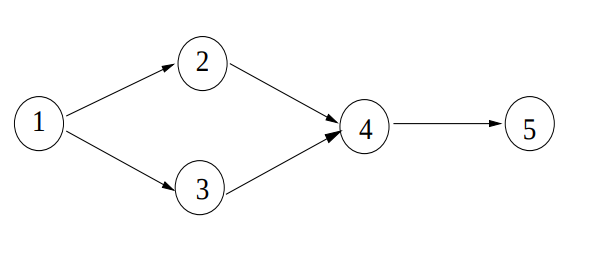
\includegraphics[scale=0.4]{img/dag_example.png}
    \centering
    \caption{Un grafo acíclico dirigido.}
    \label{fig:dag_example}
\end{figure}

En este grafo se dice que el nodo 1 es un padre de los nodos 2 y 3, y que los nodos 2 y 3 son hijos del nodo 1. La figura \ref{fig:dag_example} representa la probabilidad conjunta $p(x_1,x_2,\dots,x_5)$ para las variables aleatorias $X_1, X_2, \dots X_5$ que se puede escribir como
\[
	p(x_1,x_2,x_3,x_4,x_5) = p(x_1) p(x_2 | x_1) p(x_3 | x_1) p(x_4 | x_2, x_3) p(x_5 | x_4).
\]

En general esta relación se puede resumir como
\[
	p(x_1,x_2,\dots,x_n) = \prod_{i=1}^n p \left( x_i | \Pi_i \right),
\]
donde $\Pi_i$ denota el conjunto de variables aleatorias correspondientes a nodos padres del nodo $i$.

\subsection{Algoritmos genéticos}
Los Algoritmos Genéticos (GA por sus siglas en inglés) son métodos adaptativos que pueden ser usados para resolver problemas de búsqueda y optimización y están fuertemente inspirados en el proceso biológico de evolución. Por este motivo mucha de la terminología asociada se toma de las ciencias biológicas, sin embargo las entidades descritas por la terminología son mucho más simples que su contraparte natural. Los componentes básicos que poseen casi todos los algoritmos genéticos son:

\begin{itemize}
\item una función para evaluar la aptitud
\item una población de genomas
\item selección de los genomas aptos para reproducción
\item operación de cruza para producir la siguiente generación de genomas
\item mutación aleatoria de los genomas
\end{itemize}

En el contexto de redes bayesianas, el genoma representa la estructura del grafo dada por su matriz de adyacencia. La optimización genética se realiza evaluando los genomas por medio de una función que determine la puntuación de la red bayesiana. El motivo por el cual es necesario utilizar una búsqueda heurística en vez de una búsqueda exhaustiva tiene que ver con la cantidad posible de configuraciones de DAGs dado por la fórmula de Robinson (1977) \cite{Robinson1977} que devuelve la cantidad de grafos DAG dado un número $n$ de  vértices,
\[
	f(n) = \sum_{i=1}^n (-1)^{i+1} \binom{n}{i} 2^{i(n-i)} f(n-i).
\]
Para grafos con un número $n$ de nodos la cantidad de configuraciones posibles es:

\begin{table}[H]
\centering
\begin{tabular}{|c|c|}
\hline 
n & f(n) \\ 
\hline 
1 & 1 \\ 
\hline 
2 & 3 \\ 
\hline 
3 & 25 \\ 
\hline 
4 & 543 \\ 
\hline 
5 & 29281 \\ 
\hline 
6 & 3 781 503 \\ 
\hline 
7 & 1 138 779 265 \\ 
\hline 
8 & 783 702 329 343 \\ 
\hline 
9 & 1 213 442 454 842 881 \\ 
\hline 
\end{tabular}
\end{table}

Lo cual es imposible evaluar exhaustivamente en un tiempo razonable para una cantidad de nodos mayor a 6.

\section{Inferencia bayesiana} \label{sec:inf}
En una red bayesiana la inferencia se puede realizar evaluando múltiples posibles instancias y escogiendo aquella que maximice la probabilidad. Formalmente esto se define como
\[
	\text{Argmax}_{A,B} P(a,b | C = c) .
\]

Un ejemplo de inferencia se puede hacer sobre la red bayesiana de la figura \ref{fig:iris_graph} que representa un modelo para la base de datos Iris.

\begin{figure}[h!tb!]
    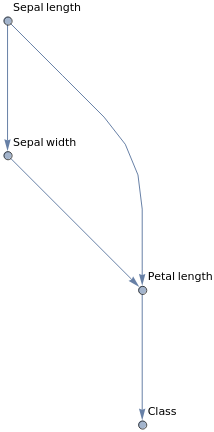
\includegraphics[scale=0.4]{img/iris_graph.png}
    \centering
    \caption{Modelo para el dataset Iris}
    \label{fig:iris_graph}
\end{figure}

Supongamos que se observa la instancia $\text{Sepal length} = 0$, $\text{Sepal width} = 2$, $\text{Petal length} = 0$, $\text{Class} = \text{Iris-setosa}$. Para calcular la probabilidad de haber observado dicha instancia bajo este modelo primero se calculan las probabilidades marginales:

\begin{figure}[H]
    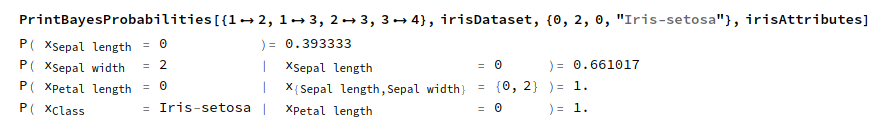
\includegraphics[scale=0.45]{img/inference_prob.png}
\end{figure}

Y posteriormente se calcula la probabilidad conjunta haciendo la multiplicación:
\[
	 P\left( x_\text{Sepal length} = 0, x_\text{Sepal width} = 2, x_\text{Petal length} = 0, x_\text{Class} = \text{Iris-setosa} \right) = 	 
\]
\[
	P(x_\text{Class} = \text{Iris-setosa} | x_\text{Petal length} = 0) \times P(x_\text{Petal length} = 0 | x_\text{Sepal length} = 0, x_\text{Sepal width} = 2)
\]
\[
	\times P(x_\text{Sepal width} = 2 | x_\text{Sepal length} = 0) \times P(x_\text{Sepal length} = 0) = 1.0 \times 1.0 \times 0.66 \times 0.39 = 0.26
\]

Para realizar una inferencia se evalúan todas las posibles sustituciones de la variable a predecir y se escoge aquella que maximice la probabilidad. Por ejemplo, para la misma red y la instancia $\text{Sepal length} = 2$, $\text{Sepal width} = 0$, $\text{Petal length} = 1$, $\text{Class} = ?$, las posibles predicciones y probabilidades son:

\begin{figure}[h!tb!]
\centering
    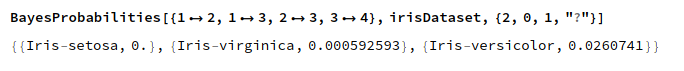
\includegraphics[scale=0.45]{img/iris_query.png}
\end{figure}

En este caso la mejor predicción de la red es que la instancia corresponde a una Iris-versicolor.

\section{Algoritmo generador de DAG} \label{sec:dag}
El objetivo a resolver en este problema es generar un algoritmo que enliste todos los posibles grafos acíclicos dirigidos (o DAG por sus siglas en inglés). Un DAG es un grafo dirigido que no posee ciclos, esto es, dado un vértice $v$ no existe ninguna secuencia de transiciones que nos regrese al mismo vértice $v$.

\begin{figure}[h!]
\centering
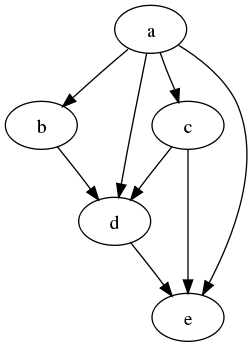
\includegraphics[scale=0.4]{img/DAG}
\caption{Ejemplo de DAG. Nótese que no existe ninguna secuencia de transiciones que comenzando desde un estado (por ejemplo el $b$), nos regrese al mismo.}
\end{figure}


\subsection{Matriz de adyacencia}
Un grafo está definido formalmente por una serie de vértices relacionados por nodos que especifican la relación entre los vértices. Sea $V$ el conjunto de vértices de un grafo, se puede construir una representación matricial del grafo a partir de una matriz cuadrada $A$ de tamaño $|V| \times |V|$ tal que sus elementos $A_{ij}$ sean $1$ cuando exista un nodo entre el $V_i$ y $V_j$, y $0$ cuando no exista.

\subsubsection*{Ejemplo}
En la figura \ref{fig:grafos} se muestra un ejemplo de grafo DAG con su respectiva representación en forma de matriz de adyacencia. Nótese que toda matriz de adyacencia estrictamente triangular superior
\[
A = \begin{cases} 
      A_{ij} & 1 < j < i \\
     0 & \text{en caso contrario} \\
    \end{cases}
\]
representa un DAG.

\begin{figure}[h!]
		\begin{subfigure}{.5\textwidth}
			\centering
			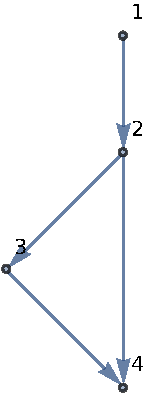
\includegraphics[scale=0.45]{img/graph}
			\caption{Grafo DAG, definido por los vértices entre los nodos.}
		\end{subfigure}%
		\begin{subfigure}{.5\textwidth}
			\centering
			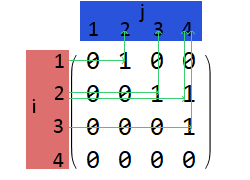
\includegraphics[scale=0.45]{img/ady_matrix}
			\caption{Representación matricial del mismo grafo.}
		\end{subfigure}%
		\caption{Ejemplo de DAG y sus representaciones.}
		\label{fig:grafos}
\end{figure}

\subsection{Representaciones equivalentes de la matriz de adyacencia de un DAG}
Debido a la forma en la que está construida la matriz de adyacencia es posible renombrar los índices de los vértices sin alterar la estructura del grafo. En la figura \ref{fig:th} se muestra el mismo grafo que en la figura \ref{fig:grafos} con la única diferencia de que se ha invertido la posición de los índices 1 y 2 en $j$. Esto no afecta a la estructura del grafo ya que la posición de los índices es sólo una convención. Se dice que dos digrafos acíclicos son isomorfos si existe un mapeo uno a uno entre ambos que preserva las relaciones de adyacencia.

\begin{figure}[h!]
\centering
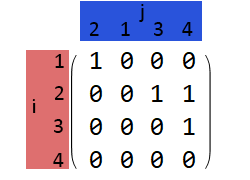
\includegraphics[scale=0.4]{img/t12v_matriz}
\caption{El mismo DAG de la figura \ref{fig:grafos} con los índices 1 y 2 en $j$ invertidos.}
\label{fig:th}
\end{figure}

La posibilidad de invertir índices sin afectar la estructura del grafo nos permite definir un conjunto de transformaciones que sobre la matriz de adyacencia que representan el mismo grafo.

\begin{definition1}
Sea $A$ una matriz que representa a un grafo, se define la función de inversión de índices $\alpha$, $\beta$ vertical como
\[
	T_{\alpha \beta V}(A) = 
	\begin{cases} 
      A_{i \beta} & j = \alpha \\
      A_{i \alpha} & j =  \beta \\
      A_{ij} & j \neq \alpha, \beta
    \end{cases}
\]
y la función de inversión de índices $\alpha$, $\beta$ horizontal como
\[
	T_{\alpha \beta H}(A) = 
	\begin{cases} 
      A_{\beta j} & i = \alpha \\
      A_{\alpha i} & i =  \beta \\
      A_{ij} & i \neq \alpha, \beta
    \end{cases}
\]
\end{definition1}
Nótese que todas las transformaciones $T$ cumplen la propiedad de linealidad
\begin{align*}
	T(A) + T(B) &= T(A+B), \\
	T(cA) &= c T(A).
\end{align*}

\subsubsection*{Ejemplo}
Si
\[
	A = \begin{pmatrix}
		a & b & c \\
		d & e & f \\
		g & h & i
	\end{pmatrix},
\]
entonces
\[
	T_{12H}(A) = \begin{pmatrix}
		b & a & c \\
		e & d & f \\
		h & g & i
	\end{pmatrix},\quad
	T_{12V}(A) = \begin{pmatrix}
		d & e & f \\
		a & b & c \\
		g & h & i
	\end{pmatrix},
\]

\subsection{Eigenvalores de la matriz de adyacencia}
Supongamos que $A$ representa la matriz de adyacencia de un grafo $G$, esto es, $A = A (G)$. $A$ sólo debe tener ceros en su diagonal, de lo contrario habría ciclos de los vértices consigo mismos. Se define $B = I + A$, la cual tiene también la propiedad de ser una matriz booleana. Si el grafo $G$ es un DAG, entonces siempre debe ser posible obtener una matriz estrictamente triangular superior por medio de una composición de transformaciones $T_{\alpha \beta V}$ y $T_{\alpha \beta H}$. Entonces los eigenvalores $\lambda$ de $B$ están dados por
\[
 \begin{vmatrix}
  1 - \lambda & x & \cdots & y \\
  0 & 1 - \lambda & \cdots & z \\
  \vdots  & \vdots  & \ddots & \vdots  \\
  0 & 0 & \cdots & 1 - \lambda 
 \end{vmatrix} = 0
\]
cuya única solución es $\lambda = 1$.

\begin{teorema1}
Sea $A$ una matriz de adyacencia que representa un grafo $G$, se define la transformación
\[
T_{\alpha \beta} (A) = T_{\alpha \beta H}(T_{\alpha \beta V}(A)) = T_{\alpha \beta V}(T_{\alpha \beta H}(A)),
\]
y la función $\operatorname{det}(A)$ que representa la determinante de $A$. Entonces
$\operatorname{det}(A) = \operatorname{det}(T_{\alpha \beta} (A))$.
\end{teorema1}

\begin{proof}
Cada operación de intercambio de filas o columnas tiene el efecto de invertir el signo de la determinante, esto es
\begin{align*}
	\operatorname{det}\left( T_{\alpha \beta H}(A) \right) &= \sum_{ijk} \epsilon_{ijk} A_{2i} A_{1j} A_{3k} \\
	&= \sum_{ijk} \epsilon_{ijk} A_{1j} A_{2i} A_{3k} \\
	&= - \sum_{jik} \epsilon_{jik} A_{1j} A_{2i} A_{3k} = - \operatorname{det}(A).
\end{align*}
Mediante un procedimiento análogo se puede probar también que
\[
	\operatorname{det}\left( T_{\alpha \beta V}(A) \right) = - \operatorname{det}(A),
\]
por lo tanto
\[
	\operatorname{det}(T_{\alpha \beta} (A)) = \operatorname{det}(A).
\]

\end{proof}
A partir de este resultado y haciendo uso de la propiedad de linealidad de las transformaciones $T$ se obtiene el siguiente corolario.
\begin{corolario}
\label{cor1}
El conjunto de transformaciones $T$ no altera los eigenvalores de la matriz de adyacencia.
\end{corolario}
\begin{proof}
Asumiendo que $T$ representa a cualquier operador del tipo $T_{\alpha \beta}$, $T_{\alpha \beta H}$ o $T_{\alpha \beta V}$, y haciendo uso de la propiedad de linealidad, se tiene que
\[
	\operatorname{eigen}(T(A)) = |T(A) - \lambda I| = |T(A-\lambda I)| = |A-\lambda I| = \operatorname{eigen}(A).
\]
\end{proof}

\subsection{Especificación de algoritmo}
El resultado del corolario \ref{cor1} nos lleva a que si $A$ representa un DAG, entonces los eigenvalores de una matriz de adyacencia de un grafo equivalente deben ser también $\lambda = 1$. Se puede comprobar fácilmente que cualquier DAG tiene una representación equivalente en forma de matriz triangular superior, por ejemplo, el DAG representado por la matriz
\[
	A = \begin{pmatrix}
		0 & 0 & 0 \\
		1 & 0 & 1 \\
		1 & 0 & 0
	\end{pmatrix}
\]
tiene una representación equivalente en forma de matriz triangular superior dada por las transformaciones
\[
	T_{12} \circ T_{13} (A) = T_{13} \circ T_{23} (A) = T_{12} \circ T_{23} (A) = \begin{pmatrix}
		0 & 1 & 1 \\
		0 & 0 & 1 \\
		0 & 0 & 0
	\end{pmatrix},
\]
en consecuencia los eigenvalores de $A+I$ son $\lambda_i (A+I) = 1$.
El algoritmo generador de DAG implementado en este proyecto genera matrices aleatorias y elimina conexiones en el grafo hasta que se cumple la condición $|\lambda_i| = 1$.

\begin{algorithm}[H]
 \KwData{tamaño grafo n}
 \KwResult{Población de matrices correspondientes a un DAG }
 Generar una población de matrices de adyacencia a partir de matrices aleatorias con elementos \{0,1\}\;
 \ForEach{Matriz de adyacencia $A_i = A(G_i)$}{
 Obtener eigenvalores $\lambda_i = \lambda(A_i)$\;
 \eIf{$|\lambda_i| = 1$}{
   $A$ representa un DAG\;
   }{
   $A$ \textbf{no} representa un DAG. Elimina conexión del grafo $G_i$ y repite\;
  }
 }
 \caption{Algoritmo generador de matrices de adyacencia DAG.}
\end{algorithm}

Este algoritmo se encuentra implementado en la función \textbf{GeneratePopulation}[\textit{n}, \textit{size}] que genera una población de tamaño \textit{size} con un número \textit{n} de atributos.

\begin{figure}[h!tb!]
\centering
    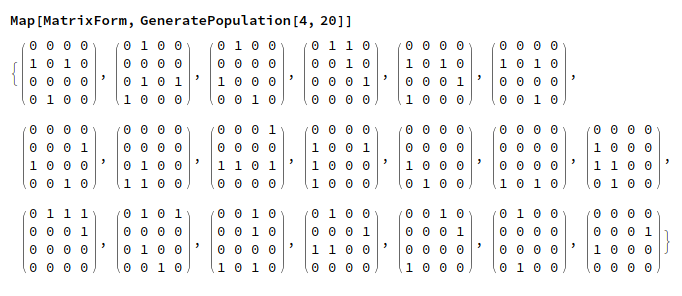
\includegraphics[scale=0.45]{img/population_gen.png}
\end{figure}

\section{Métrica MDL} \label{sec:mdl}
El principio de \textit{longitud de mínima descripción} (minimum description length o MDL) afirma que el mejor modelo es aquel que permite la descripción más corta, en el contexto de la codificación de los datos y el modelo mismo \cite{MDL}. La longitud de descripción el el número de bits requeridos para almacenar tal codificación.

La métrica se descompone en varios subcomponentes que dan lugar a la descripción completa del modelo.

\subsection{Codificación de las variables} 
Primero se codifica el número de variables y el número posible de valores que puede tomar cada una. El número de posibles valores que puede tomar la variable aleatoria $X_i$ se denota por $\| X_i \|$.

\[
	DL_{var} = \log n + \sum_{i=1}^n \log \| X_i \|
\]

\subsection{Codificación del DAG}
Se puede describir el DAG guardando para cada variable desde $X_1$ hasta $X_n$ el número de padres y una lista de padres. Dado que $\Pi_i$ denota el conjunto de padres de $X_i$, entonces $|\Pi_i|$ se usa para denotar el número de padres de $X_i$. 

\[
	DL_{dag} = \sum_{i=1}^n \left( 1 + |\Pi_i| \right) \log n
\]

\subsection{Codificación de los parámetros}
En la red bayesiana hay un parámetro por cada posible combinación de probabilidad condicional y posibles valores de las variables. Para esto se cuentan las posibles configuraciones $\| \Pi_i \|$ de los padres del nodo $X_i$ y todos los $\| X_i \|$ posibles valores del nodo.

\[
	DL_{param} = \frac{1}{2} \log m \sum_{i=1}^n \| \Pi_i \| \left( \| X_i \| - 1 \right)
\]

\subsection{Codificación de los datos}
Los datos consisten en una secuencia $m$ de realizaciones de $U = \left( X_1, X_2, \dots, X_n \right)$. Usando la codificación de Shannon la contribución de los datos es:
\[
	DL_{data} = - \sum_{i=1}^m \log p(u_i)
\]

\subsection{MDL}
La puntuación MDL se define como la longitud total de descripción del modelo y los datos.
\[
	MDL = DL_{var} + DL_{dag} + DL_{param} + DL_{data}
\]

El cálculo de la puntuación MDL se encuentra implementado en la función \textbf{MDLScore}[\textit{dag}, \textit{dataset}], donde \textit{dag} es una lista de conexiones del grafo y \textit{dataset} es la lista de instancias. Nótese que el valor del MDL de un modelo con estructura no trivial:
\begin{figure}[H]
\centering
    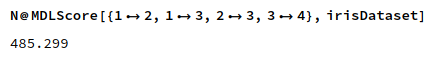
\includegraphics[scale=0.45]{img/iris_mdl.png}
\end{figure}
es menor que un modelo vacío:
\begin{figure}[H]
\centering
    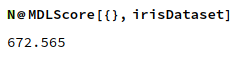
\includegraphics[scale=0.45]{img/iris_mdl_empty.png}
\end{figure}

\section{Evaluación de aptitud} \label{sec:apt}
Existen múltiples esquemas para particionar los datos en conjuntos de entrenamiento y prueba con diferentes propiedades. En este trabajo se utilizaron tres:
\begin{itemize}
	\item Evaluación con mismos datos de entrenamiento y prueba.
	\item Evaluación con minibatches.
	\item Evaluación con validación cruzada.
\end{itemize}

La evaluación con mismos datos de entrenamiento y prueba es lo más rápido pero puede generar modelos que sobreajusten los datos y que tengan poca capacidad predictiva. La evaluación con minibatches consiste en entrenar y evaluar con subconjuntos aleatorios de la base de datos. Esto es útil si la base de datos es demasiado grande. Por último el esquema de validación cruzada consiste en hacer múltiples particiones a los datos como se muestra en la figura \ref{fig:crossvalidation} y entrenar seleccionando las particiones correspondientes a cada iteración.

\begin{figure}[h!tb!]
\centering
    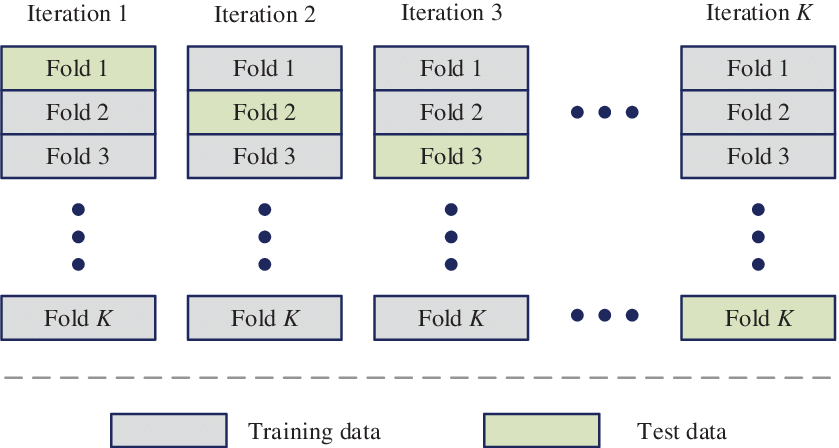
\includegraphics[scale=0.35]{img/cross-validation.png}
    \caption{Diagrama del algoritmo de validación cruzada.}
    \label{fig:crossvalidation}
\end{figure}

Esto se implementó en las funciones \textbf{EvaluateGenome}, \textbf{EvaluateGenomeWithMinibatch} y \textbf{EvaluateGenomeWithKFolds}. Un ejemplo de uso es:

\begin{figure}[h!tb!]
\centering
    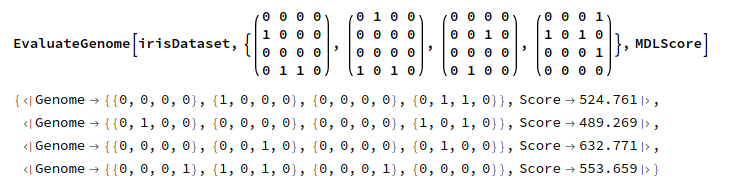
\includegraphics[scale=0.45]{img/evaluate_iris.png}
\end{figure}

\section{Optimización genética} \label{sec:gen}

\subsection{Selección de población}

La selección se hace de manera aleatoria y proporcional, dando preferencia a los individuos más aptos. El algoritmo de selección ordena los individuos según su aptitud escoge un índice aleatorio con mayor peso en los individuos más aptos.

\textbf{ProportionateSelection}[\textit{population}, \textit{n}, \textit{selectionCriteria}] realiza la selección a partir de la población evaluada \textit{population}, tomando \textit{n} individuos con el criterio de selección \textit{selectionCriteria} que puede tomar los valores "LessIsBetter" o "MoreIsBetter".

\begin{figure}[h!tb!]
\centering
    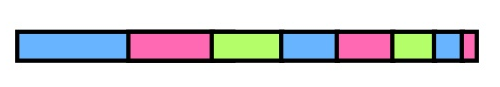
\includegraphics[scale=0.45]{img/selection_diagram.png}
\end{figure}

\subsection{Operador de cruza}
La cruza se realiza de manera aleatoria, seleccionando un valor de cualquiera de ambos padres haciendo un muestreo aleatorio. \textbf{PopulationCrossover}[\textit{population}, \textit{childrenPerCouple}] realiza la cruza emparejando aleatoriamente pares de individuos dentro de la población produciendo \textit{childrenPerCouple} hijos por cada par.

\begin{figure}[h!tb!]
\centering
    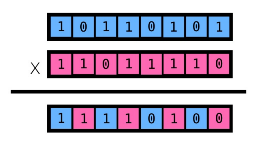
\includegraphics[scale=0.45]{img/crossover_diagram.png}
\end{figure}

\subsection{Mutación}
La mutación se realiza cambiando un solo elemento del genoma en una posición aleatoria. \textbf{PopulationMutate}[\textit{population},\textit{probability}] aplica mutationes aleatoriamente con una probabilidad \textit{probability} sobre cada individuo de la población. Sólo un alelo es modificado por cada mutación.

\begin{figure}[h!tb!]
\centering
    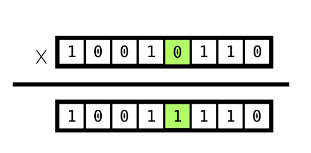
\includegraphics[scale=0.45]{img/mutation_diagram.png}
\end{figure}

\section{Resultados} \label{sec:results}
Como resultado se obtiene una interfaz de usuario que permite encontrar la mejor estructura. \textbf{GenerateInitialPopulation}[\textit{size}, \textit{dataset}, \textit{opts}] genera una población inicial de una cantidad \textit{size} de individuos y evalúa su rendimiento en la base de datos \textit{dataset}. Sus posibles argumentos opcionales son:
\begin{itemize}
\item \textit{ScoringFunction} que puede tomar los valores \textit{MDL} para evaluar usando la métrica MDL y \textit{CorrectlyClassified} para evaluar usando la métrica de porcentaje de instancias correctamente evaluadas.
\item \textit{TestMethod} puede tomar los valores \textit{UseTrainingSet} para evaluar usando el mismo conjunto de datos de entrenamiento, \textit{UseMiniBatch} para evaluar por medio de minibatches de tamaño especificado en la opción \textit{MiniBatchSize}, y \textit{KFoldCrossValidation} para evaluar usando validación cruzada de n pliegues especificados en la opción Folds.
\item \textit{MiniBatchSize} es el tamaño del minibatch. Por defecto no está especificado, por lo que es necesario introducir esta opción explicitamente si se especifica TestMethod $\rightarrow$ UseMiniBatch.
\item \textit{Folds} es el número de pliegues en la validación cruzada. Por defecto tiene el valor de 10.
\end{itemize}

\textbf{Generation}[\textit{dataset}, \textit{population}, \textit{survivors}, \textit{mutationProb}, opts] realiza una generación del algoritmo genético con la población \textit{population}, el número de sobrevivientes \textit{survivors}, y la probabilidad de mutación \textit{mutationProb}. Sus posibles argumentos opcionales son: 
\begin{itemize}
\item \textit{ScoringFunction}, \textit{TestMethod}, \textit{MiniBatchSize} y \textit{Folds} usados en la función \textbf{GenerateInitialPopulation}, y
\item \textit{ScoreType} que especifica la preferencia del algoritmo de selección proporcional, y puede tomar los valores \textit{LessIsBetter} para dar preferencia a puntuaciones con menor valor y \textit{MoreIsBetter} para dar preferencia a puntuaciones con mayor valor.
\end{itemize}

\textbf{GeneticOptimize}[\textit{dataset, population, survivors, mutationProb, generations}, opts] realiza una cantidad \textit{generations} de iteraciones del algoritmo evolutivo.

También se implementaron funciones auxiliares para visualización de resultados:
\begin{itemize}
\item \textbf{SelectBest}[\textit{population, n, scoreType}] selecciona los \textit{n} individuos más aptos de la población de acuerdo al criterio \textit{scoreType}.
\item \textbf{PlotBayesNet}[\textit{net, attributes}] grafica la red bayesiana.
\item \textbf{PlotGeneration}[\textit{generation, attributes, index}] grafica los individuos de una generación en la iteración especificada en \textit{index}.
\item \textbf{PopulationCorrectlyClassifiedPercentage}[\textit{population, testData}] calcula el porcentaje de aciertos promedio de una población sobre una base de datos de prueba.
\end{itemize}

Las figuras \ref{fig:iris_results}, \ref{fig:car_results}, \ref{fig:bank_results}, \ref{fig:adult_results}, \ref{fig:servo_results} y \ref{fig:tic-tac-toe_results} muestran los resultados del proceso de entrenamiento para las bases de datos Iris, Car, Bank, Adult, Servo y Tic-Tac-Toe obtenidas del UCI Dataset.

\begin{figure}[htb!]
          \begin{subfigure}[b]{0.48\textwidth}
            \centering 
            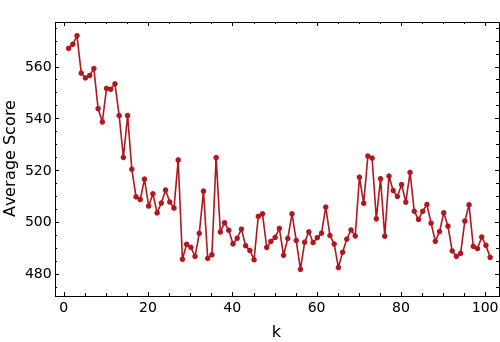
\includegraphics[width=\textwidth]{img/iris/ScoreVsK.png}
            \caption[ ]{{Puntuación MDL por generación.}}
          \end{subfigure}
                  \hfill
          \begin{subfigure}[b]{0.48\textwidth}
            \centering 
            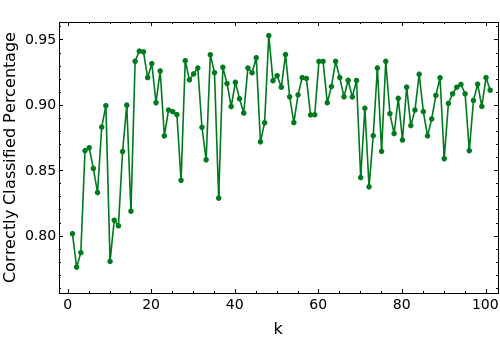
\includegraphics[width=\textwidth]{img/iris/CorrectlyClassifiedVsK.png}
            \caption[ ]{{Porcentaje de instancias correctamente clasificadas por generación.}}
          \end{subfigure}
                  \vskip\baselineskip
        \centering
        \begin{subfigure}[b]{0.475\textwidth}
            \centering
            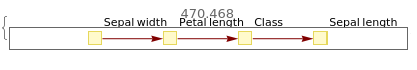
\includegraphics[width=\textwidth]{img/iris/first.png}
            \caption[ ]{{Primera generación.}}
        \end{subfigure}
        \hfill
        \begin{subfigure}[b]{0.475\textwidth}
            \centering 
            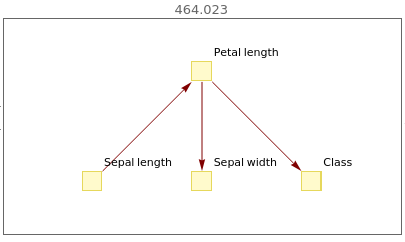
\includegraphics[width=\textwidth]{img/iris/best.png}
            \caption[ ]{{Estructura óptima alcanzada en la generación 100.}}
        \end{subfigure}

\caption{Resultados para la base de datos Iris.}
\label{fig:iris_results}
\end{figure}

\begin{figure}[htb!]
          \begin{subfigure}[b]{0.48\textwidth}
            \centering 
            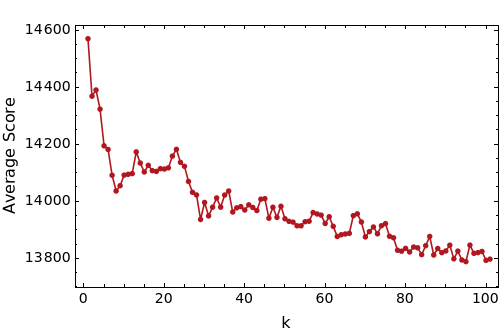
\includegraphics[width=\textwidth]{img/car/ScoreVsK.png}
            \caption[ ]{{Puntuación MDL por generación.}}
          \end{subfigure}
                  \hfill
          \begin{subfigure}[b]{0.48\textwidth}
            \centering 
            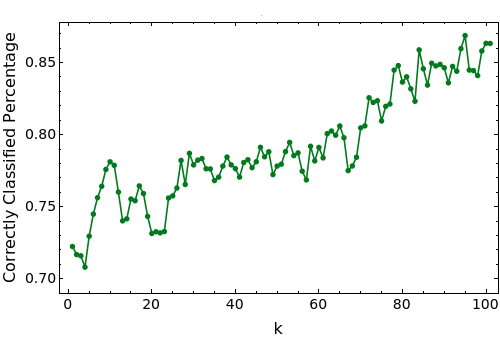
\includegraphics[width=\textwidth]{img/car/CorrectlyClassifiedVsK.png}
            \caption[ ]{{Porcentaje de instancias correctamente clasificadas por generación.}}
          \end{subfigure}
                  \vskip\baselineskip
        \centering
        \begin{subfigure}[b]{0.475\textwidth}
            \centering
            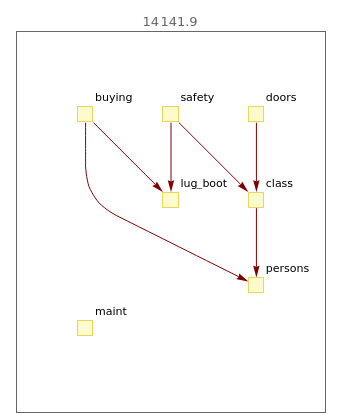
\includegraphics[width=\textwidth]{img/car/first.png}
            \caption[ ]{{Primera generación.}}
        \end{subfigure}
        \hfill
        \begin{subfigure}[b]{0.475\textwidth}
            \centering 
            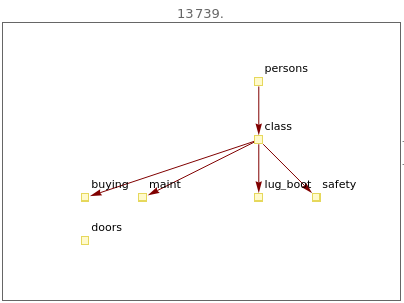
\includegraphics[width=\textwidth]{img/car/best.png}
            \caption[ ]{{Estructura óptima alcanzada en la generación 100.}}
        \end{subfigure}

\caption{Resultados para la base de datos Car.}
\label{fig:car_results}
\end{figure}

\begin{figure}[htb!]
          \begin{subfigure}[b]{0.48\textwidth}
            \centering 
            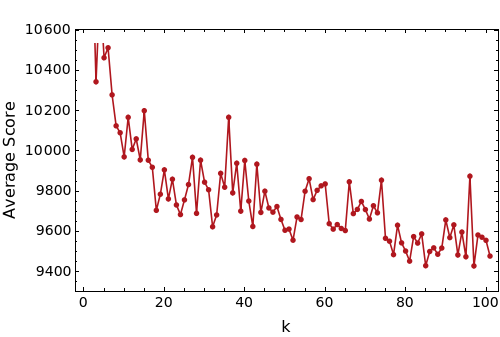
\includegraphics[width=\textwidth]{img/bank/ScoreVsK.png}
            \caption[ ]{{Puntuación MDL por generación.}}
          \end{subfigure}
                  \hfill
          \begin{subfigure}[b]{0.48\textwidth}
            \centering 
            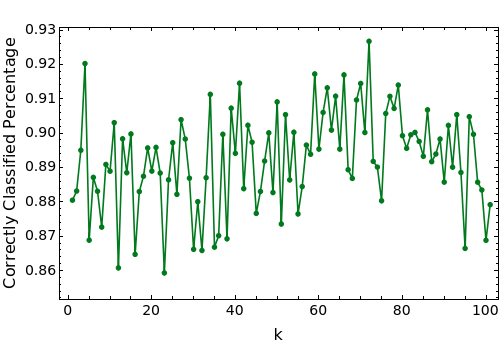
\includegraphics[width=\textwidth]{img/bank/CorrectlyClassifiedVsK.png}
            \caption[ ]{{Porcentaje de instancias correctamente clasificadas por generación.}}
          \end{subfigure}
                  \vskip\baselineskip
        \centering
        \begin{subfigure}[b]{0.475\textwidth}
            \centering
            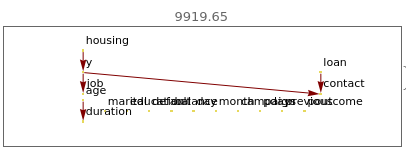
\includegraphics[width=\textwidth]{img/bank/first.png}
            \caption[ ]{{Primera generación.}}
        \end{subfigure}
        \hfill
        \begin{subfigure}[b]{0.475\textwidth}
            \centering 
            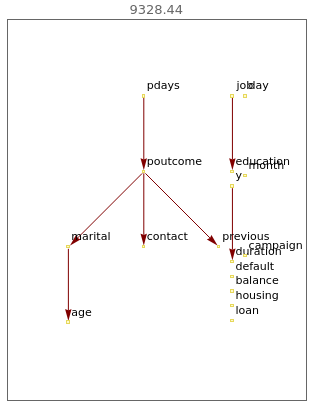
\includegraphics[width=\textwidth]{img/bank/best.png}
            \caption[ ]{{Estructura óptima alcanzada en la generación 100.}}
        \end{subfigure}

\caption{Resultados para la base de datos Bank.}
\label{fig:bank_results}
\end{figure}

\begin{figure}[htb!]
          \begin{subfigure}[b]{0.48\textwidth}
            \centering 
            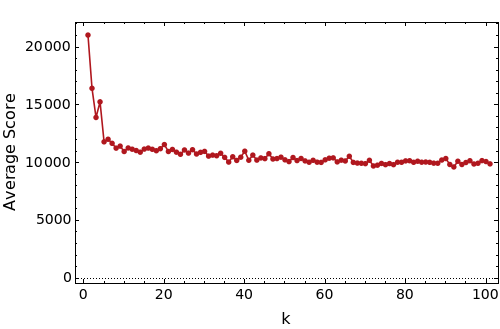
\includegraphics[width=\textwidth]{img/adult/ScoreVsK.png}
            \caption[ ]{{Puntuación MDL por generación.}}
          \end{subfigure}
                  \hfill
          \begin{subfigure}[b]{0.48\textwidth}
            \centering 
            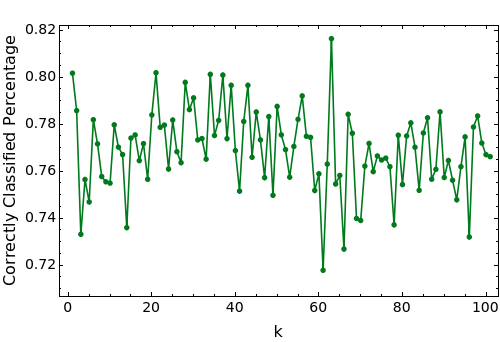
\includegraphics[width=\textwidth]{img/adult/CorrectlyClassifiedVsK.png}
            \caption[ ]{{Porcentaje de instancias correctamente clasificadas por generación.}}
          \end{subfigure}
                  \vskip\baselineskip
        \centering
        \begin{subfigure}[b]{0.475\textwidth}
            \centering
            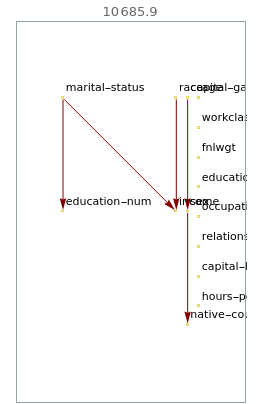
\includegraphics[width=\textwidth]{img/adult/first.png}
            \caption[ ]{{Primera generación.}}
        \end{subfigure}
        \hfill
        \begin{subfigure}[b]{0.475\textwidth}
            \centering 
            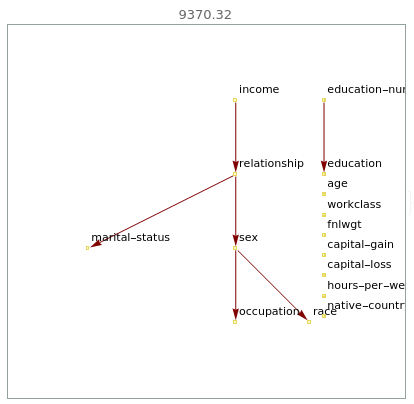
\includegraphics[width=\textwidth]{img/adult/best_73.png}
            \caption[ ]{{Estructura óptima alcanzada en la generación 73.}}
        \end{subfigure}

\caption{Resultados para la base de datos Adult.}
\label{fig:adult_results}
\end{figure}

\begin{figure}[htb!]
          \begin{subfigure}[b]{0.48\textwidth}
            \centering 
            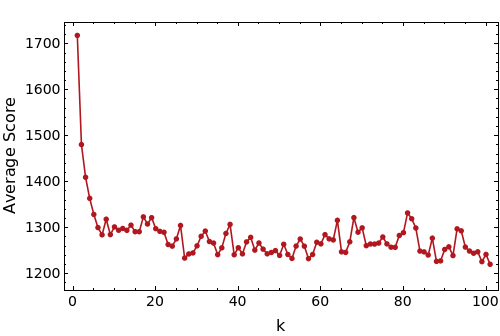
\includegraphics[width=\textwidth]{img/servo/ScoreVsK.png}
            \caption[ ]{{Puntuación MDL por generación.}}
          \end{subfigure}
                  \hfill
          \begin{subfigure}[b]{0.48\textwidth}
            \centering 
            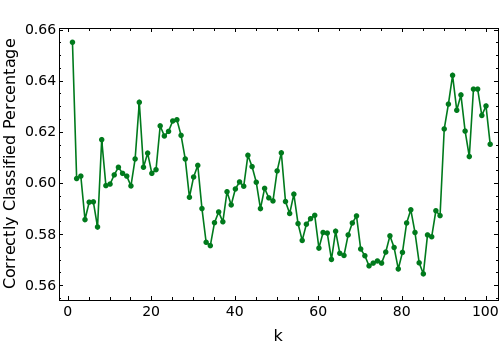
\includegraphics[width=\textwidth]{img/servo/CorrectlyClassifiedVsK.png}
            \caption[ ]{{Porcentaje de instancias correctamente clasificadas por generación.}}
          \end{subfigure}
                  \vskip\baselineskip
        \centering
        \begin{subfigure}[b]{0.475\textwidth}
            \centering
            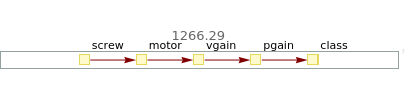
\includegraphics[width=\textwidth]{img/servo/first.png}
            \caption[ ]{{Primera generación.}}
        \end{subfigure}
        \hfill
        \begin{subfigure}[b]{0.475\textwidth}
            \centering 
            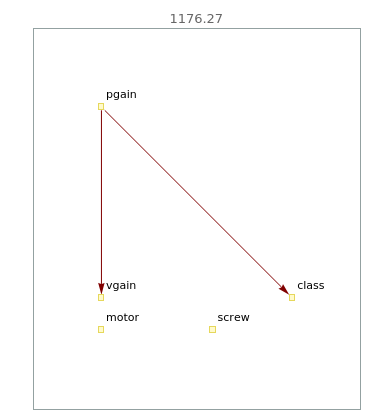
\includegraphics[width=\textwidth]{img/servo/best.png}
            \caption[ ]{{Estructura óptima alcanzada en la generación 100.}}
        \end{subfigure}

\caption{Resultados para la base de datos Servo.}
\label{fig:servo_results}
\end{figure}

\begin{figure}[htb!]
          \begin{subfigure}[b]{0.48\textwidth}
            \centering 
            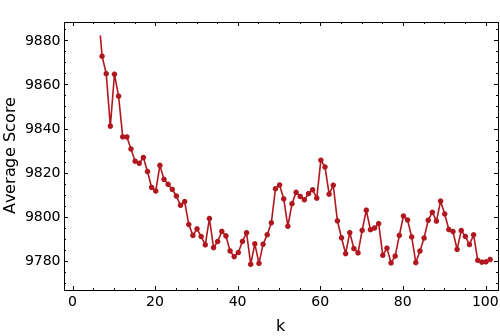
\includegraphics[width=\textwidth]{img/tic-tac-toe/ScoreVsK.png}
            \caption[ ]{{Puntuación MDL por generación.}}
          \end{subfigure}
                  \hfill
          \begin{subfigure}[b]{0.48\textwidth}
            \centering 
            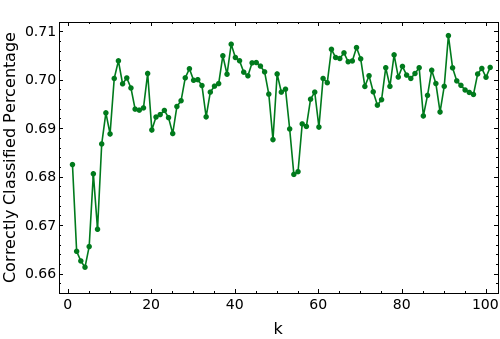
\includegraphics[width=\textwidth]{img/tic-tac-toe/CorrectlyClassifiedVsK.png}
            \caption[ ]{{Porcentaje de instancias correctamente clasificadas por generación.}}
          \end{subfigure}
                  \vskip\baselineskip
        \centering
        \begin{subfigure}[b]{0.475\textwidth}
            \centering
            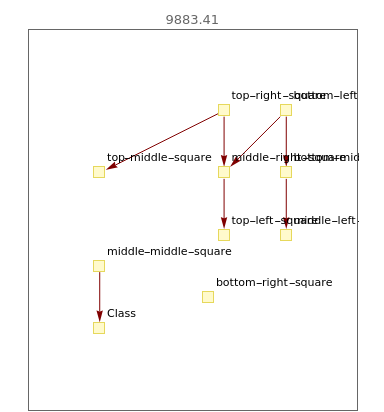
\includegraphics[width=\textwidth]{img/tic-tac-toe/first.png}
            \caption[ ]{{Primera generación.}}
        \end{subfigure}
        \hfill
        \begin{subfigure}[b]{0.475\textwidth}
            \centering 
            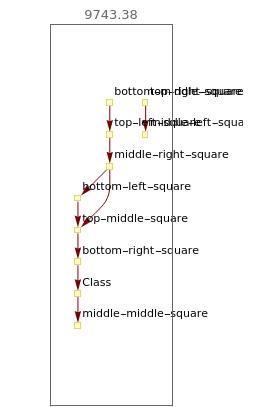
\includegraphics[width=\textwidth]{img/tic-tac-toe/best.png}
            \caption[ ]{{Estructura óptima alcanzada en la generación 100.}}
        \end{subfigure}

\caption{Resultados para la base de datos Tic-Tac-Toe.}
\label{fig:tic-tac-toe_results}
\end{figure}

\clearpage
\nocite*
\bibliography{Referencias}{}
\bibliographystyle{plain}

\end{document}